%%%% using 'arara' 4.0
% arara: xelatex: {synctex: yes, interaction: nonstopmode}
% arara: bibtex
% arara: xelatex: {synctex: yes, interaction: nonstopmode}
% arara: xelatex: {synctex: yes, interaction: nonstopmode}

% arara: indent: {overwrite: yes}

% arara: clean: { extensions: [aux, bcf, cod, blg, lof, lot, out, toc, log, xml, bak0 ] }

\documentclass[review]{elsarticle}

% Figures Links, mittig und rechts platzieren
\usepackage[export]{adjustbox}
\usepackage{caption}
\usepackage{subcaption}
\usepackage{amsmath}

% prevents that appendices are moved behind references
\usepackage{placeins}

\usepackage[nolist]{acronym}

\usepackage{longtable}
\usepackage{booktabs}
\usepackage{multirow}
\usepackage{float}

\graphicspath{{../03_figures/results/}{./}{../03_figures/data/}} 

% enable paragraph as 4th level https://tex.stackexchange.com/questions/60209/how-to-add-an-extra-level-of-sections-with-headings-below-subsubsection
\usepackage{titlesec}
\setcounter{secnumdepth}{4}
\titleformat{\paragraph}
{\normalfont\small\bfseries}{\theparagraph}{1em}{}
\titlespacing*{\paragraph}
{0pt}{3.25ex plus 1ex minus .2ex}{1.5ex plus .2ex}

% enable linking to subsubsection
\setcounter{secnumdepth}{3}

% various symbols, e.g. \degree
\usepackage{gensymb}

\usepackage[hidelinks]{hyperref}

\usepackage{lineno}
\modulolinenumbers[5]

% set autoref abbr for appendix
\newcommand*{\Appendixautorefname}{appendix}

\journal{Journal "Remote Sensing of Environment"}

% line breaks in table cells
\newcommand{\specialcell}[2][l]{%
  \begin{tabular}[#1]{@{}l@{}}#2\end{tabular}}

% tilde
\newcommand{\mytilde}{\raise.17ex\hbox{$\scriptstyle\mathtt{\sim}$}}

%% APA style
\bibliographystyle{model5-names}\biboptions{authoryear}

\begin{document}

\begin{frontmatter}

	\title{title}

	%% Group authors per affiliation:
	\author[FSU]{Patrick Schratz}
	\cortext[mycorrespondingauthor]{Corresponding author}
	\ead{patrick.schratz@uni-jena.de}

	\author[FSU]{Jannes Muenchow}
	\author[NEIKER]{Eugenia Iturritxa}
	%\author[TUDO]{Jakob Richter}
	\author[FSU]{Alexander Brenning}

	\address[FSU]{Department of Geography, GIScience group, Grietgasse 6, 07743, Jena, Germany}
	%\address[NEIKER]{NEIKER, Granja Modelo –Arkaute, Apdo. 46, 01080 Vitoria-Gasteiz, Arab, Spain}
	%\address[TUDO]{Department of Statistics, TU Dortmund University, Germany}

	\begin{abstract}

	\end{abstract}

	\begin{keyword}
		hyperspectral imagery \sep penalized regression \sep machine-learning \sep variable importance \sep spatial cross-validation
	\end{keyword}

\end{frontmatter}

\linenumbers

% längste Abkürzung steht hier!!! in eckigen Klammern
\begin{acronym}[AUROC]

	% geringerer Zeilenabstand
	%\setlength{\itemsep}{-\parsep}
	\acro{ANN}{Artificial Neural Network}
	\acro{AUROC}{Area Under the Receiver Operating Characteristics Curve}
	\acro{BRT}{Boosted Regression Trees}
	\acro{CART}{Classification and Regression Trees}
	\acro{CV}{cross-validation}
	\acro{ENM}{Environmental Niche Modeling}
	\acro{FPR}{False Positive Rate}
	\acro{GAM}{Generalized Additive Model}
	\acro{GBM}{Gradient Boosting Machine}
	\acro{GLM}{Generalized Linear Model}
	\acro{ICGC}{Institut Cartografic i Geologic de Catalunya}
	\acro{IQR}{Interquartile Range}
	\acro{WKNN}{Weighted $k$-nearest neighbor}
	\acro{MARS}{Multivariate Adaptive Regression Splines}
	\acro{MEM}{Maximum Entropy Model}
	\acro{NRI}{Normalized Ratio Index}
	\acro{OLS}{Ordinary Least Squares}
	\acro{LOWESS}{Locally Weighted Scatter Plot Smoothing}
	\acro{PISR}{Potential Incoming Solar Radiation}
	\acro{RBF}{Radial Basis Function}
	\acro{RF}{Random Forest}
	\acro{RMSE}{Root Mean Square Error}
	\acro{RR}{Ridge Regression}
	\acro{RSS}{Residual Sum of Squares}
	\acro{SDM}{Species Distribution Modeling}
	\acro{SVM}{Support Vector Machines}
	\acro{TPR}{True Positive Rate}
\end{acronym}

\section{Introduction}
\label{sec:intro}

\section{Data and study area}

\subsection{In-situ data}
% Describe Plots

The four \textit{Pinus radiata} plots Laukiz 1, Laukiz 2, Luiando and Oiartzun are located in the northern part of the Basque Country (\autoref{fig:study_area}).
Oiartzun has the most observations (n = 529) while Laukiz 2 has largest area size.
All plots besides Luiando are located nearby the coast.
The data was collected in September 2016.

\begin{figure} [t!]
	\begin{center}
		\makebox[\textwidth]{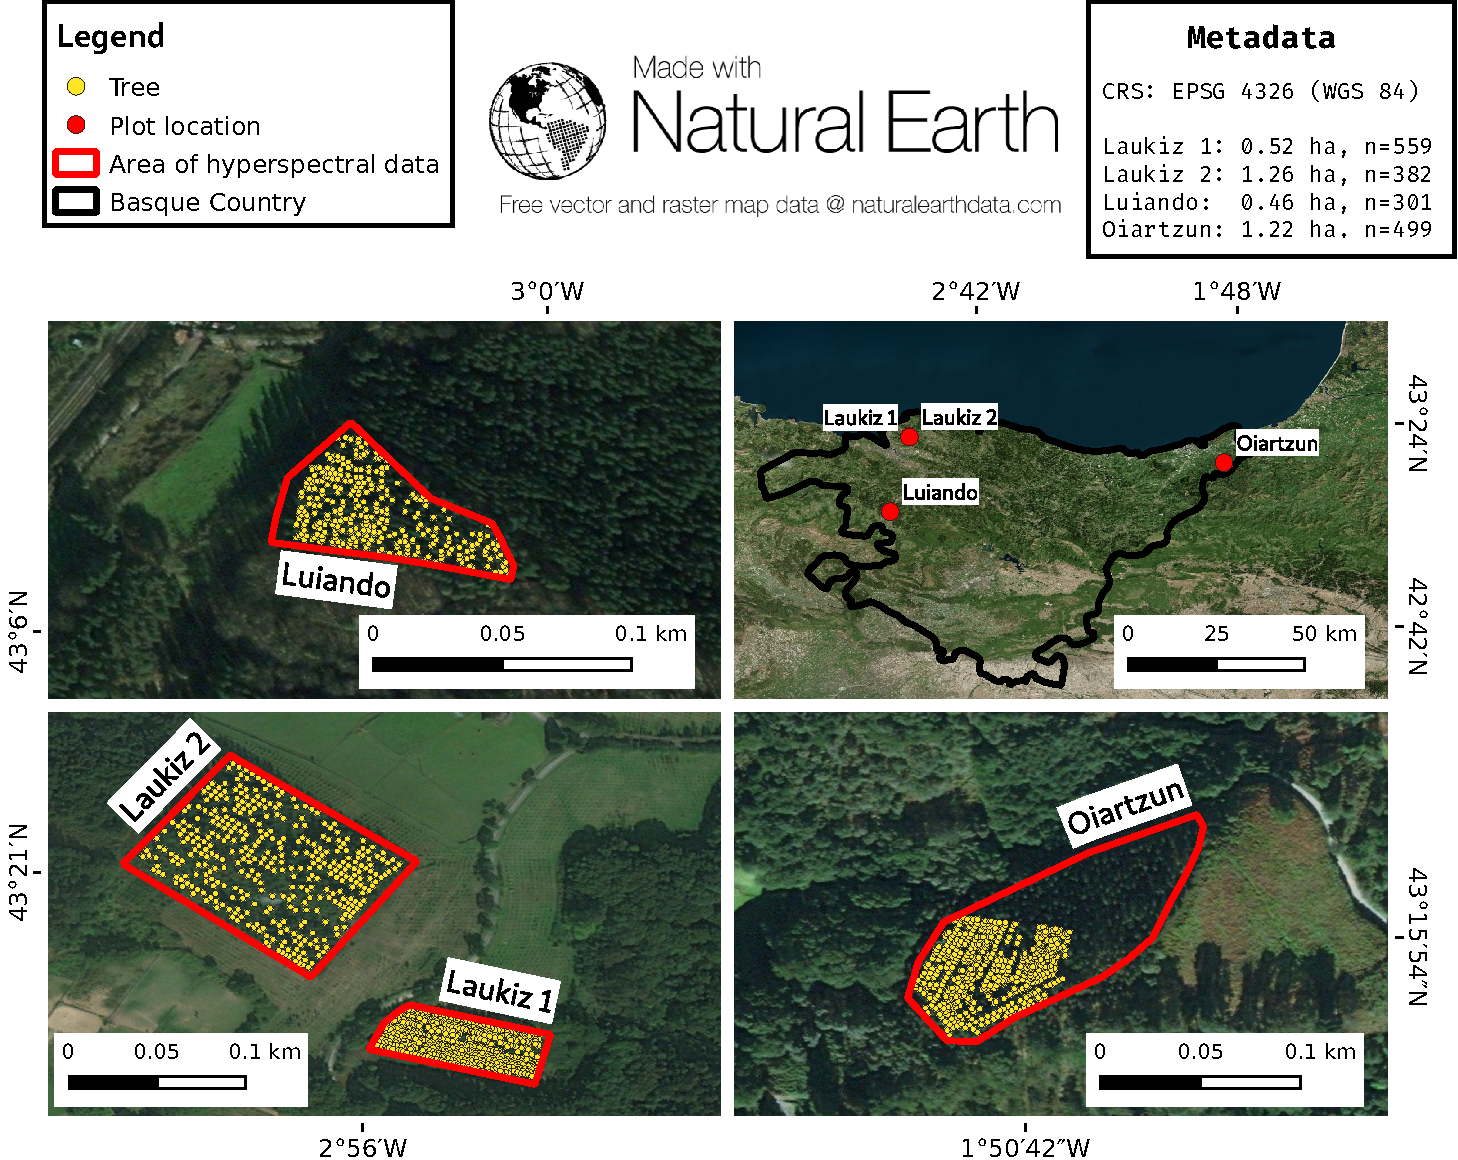
\includegraphics[width=\textwidth] {study_area_hyperspectral.pdf}}
		\caption{Information about the plot locations, the area of hyperspectral coverage and the number of trees per plot.}
		\label{fig:study_area}
	\end{center}
\end{figure}

\subsection{Hyperspectral data}

The airborne hyperspectral data was acquired during two flight campaigns on September 28th and October 5th 2016, both around 12 am.
The images were taken by an AISAEAGLE-II sensor from the \ac{ICGC}.
All preprocessing steps (geometric, radiometric, atmospheric) have been conducted by \ac{ICGC}.

Additional information is provided in Table 1:

% parameter limits
\begin{table}[b!]
\centering
\caption[t]{Specifications of hyperspectral data.}
\begingroup\footnotesize
\begin{tabular}{ll}
	\\
	Characteristic         & Value                               \\
	\hline
	Geometric resolution   & 1 m                                 \\
	Radiometric resolution & 12 bit                              \\
	Spectral resolution    & 126 bands (404.08 nm - 996.31 nm)   \\
	Correction:            & Radiometric, geometric, atmospheric
\end{tabular}
\endgroup
\label{tab:hyperparameter_limits}
\end{table}

\section{Methods}

\subsection{Derivation of indices}

% link to PDF with veg indices
All vegetation indices (90 total) suitable for the wavelength range of the hyperspectral data and offered by the \texttt{hsdar} package have been calculated.
Additionally, all possible \ac{NRI} were calculated from the data using the formula:

\begin{equation}
	NRI_{i,j} = \frac{b_{i} - b_{j}}{b_{i} + b_{j}}
\end{equation}

\noindent
where $i$ and $j$ are the respective band numbers.

%To account for geometric offsets, we calculated every index five times using a buffer from 1 - 5 meter around the centroid of the respective tree.
To account for geometric offsets, we used a buffer of 2 meters around the centroid of the respective tree.
The mean value of all pixels touched by the buffer was assigned as the final value for each index.
Missing values were removed from the mean value calculation.
In total, 7875 Normalized Ratio Indices NRI have been calculated ($\frac{125*126}{2}$).
Some indices returned \texttt{NA} values for some observations and were removed from the dataset, leaving a total of 7471 variables without missing values.

\subsection{Exploratory plot characteristics}

To get a better impression on the infection state of the four plots, an exploratory data analysis was done.
The distribution of the response variable \texttt{defoliation} was visualized as well as the spectral signatures of each plot.

\subsection{Benchmarking of algorithms}

Multiple algorithms were benchmarked on predictive performance to find the best performing one.
Besides well-known machine-learning algorithms like \ac{RF} and \ac{SVM} we also used \textit{xgboost} due to its promising results in recent machine-learning competitions.
To expand the algorithm selection even more, we also used penalized L2 (Ridge) regression.
This algorithm is able to account for the high correlation between the predictors by penalizing the estimated coefficients of the fitted model.

\subsubsection{The ridge penalty}

In \ac{RR} (also called $\ell_{2}$ penalization) the assumption of unbiased coefficients is given up in favor of higher predictive accuracy and reduced variance \citep{Hastie2001}.
Coefficients are standardized and penalized for their size.
When minimizing the \ac{RSS}, \ac{RR} adds a penalization term $\lambda \sum_{j=1}^{p}\beta_{j}^{2}$ to the equation:

\begin{equation}
	RSS = \sum_{i=1}^{n} \left(y_{i} - \beta_{0} - \sum_{j=1}^{p} \beta_{j} x_{ij} \right) ^{2} + \lambda \sum_{j=1}^{p}\beta_{j}^{2}
\end{equation}

where $\lambda >= 0$ is a tuning parameter responsible for the magnitude of penalization.
To make the second term (usually referred to as the \textit{shrinkage penalty}) of this equation small, the coefficients $\beta_{j}$ need to become small.
Unlike to Lasso however, predictors are not removed from the final model and will always be $\beta_{j} >= 0$.
Hence, $\lambda$ has the effect of shrinking the coefficients when minimizing the \ac{RSS}.
For $\lambda = 0$, no penalization is done and standard \ac{OLS} applies \citep{James2013}.
The \textit{shrinkage penalty} is only applied to the coefficients and not to the intercept.
Also, while \ac{OLS} generates only one set of coefficient estimates, \ac{RR} will create multiple sets for every value of $\lambda$.
In summary, the advantage of \ac{RR} is based on the bias-variance tradeoff: For $\lambda\to\infty$, the flexibility of the fit is reduced leading to a decrease in variance of the coefficients but also introduces a (substantial) bias.
For $\lambda = 0$, the variance is high but coefficients are unbiased \citep{James2013}.

\subsubsection{Performance estimation}

The algorithms were benchmarked using a spatial \ac{CV} on the plot level.
The dataset was split into four folds, each fold representing one plot.
Algorithms were trained on three out of four plots and evaluated on the remaining plot.
Hyperparameter tuning was also performend on the plot level: Each respective training set, consisting of observations from three plots, was again split into three partitions to estimate the best performing hyperparameter set.

% figure visualizing the folds

\subsection{Variable importance}

We aimed to find indices that contribute most when predicting defoliation.
Permutation-based variable importance was applied on the best performing algorithm.

% partial dependence plots??


\section{Results}

% Performance estimates
\begin{table}[b!]
\centering
\caption[t]{Four-fold spatial \ac{CV} performances of RF, RR, SVM and xgboost using \ac{RMSE} as the error measure. 
Mean and standard deviation are shown.}
\begingroup\footnotesize
\begin{tabular}{llll}
	\\
	RF            & RR            & SVM           & xgboost \\
	\hline
	54.80 (17.58) & 53.67 (17.95) & 54.66 (17.67) &         \\
	\bottomrule
\end{tabular}
\endgroup
\label{tab:penalty_comparison}
\end{table}

\section{Results}

\subsection{Exploratory data analysis}

% defoliation boxplots
\begin{figure} [t!]
	\begin{center}
		\makebox[\textwidth]{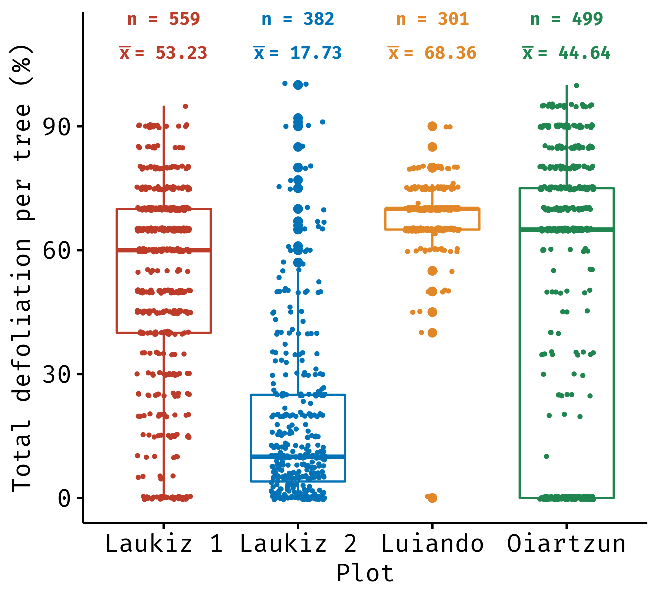
\includegraphics[width=0.7\textwidth] {../03_figures/results/boxplot_defol.pdf}}
		\caption{Descriptive statistics of the response variable \textit{defoliation}.}
		\label{fig:defol_boxplots}
	\end{center}
\end{figure}

% spectral signatures
\begin{figure} [t!]
	\begin{center}
		\makebox[\textwidth]{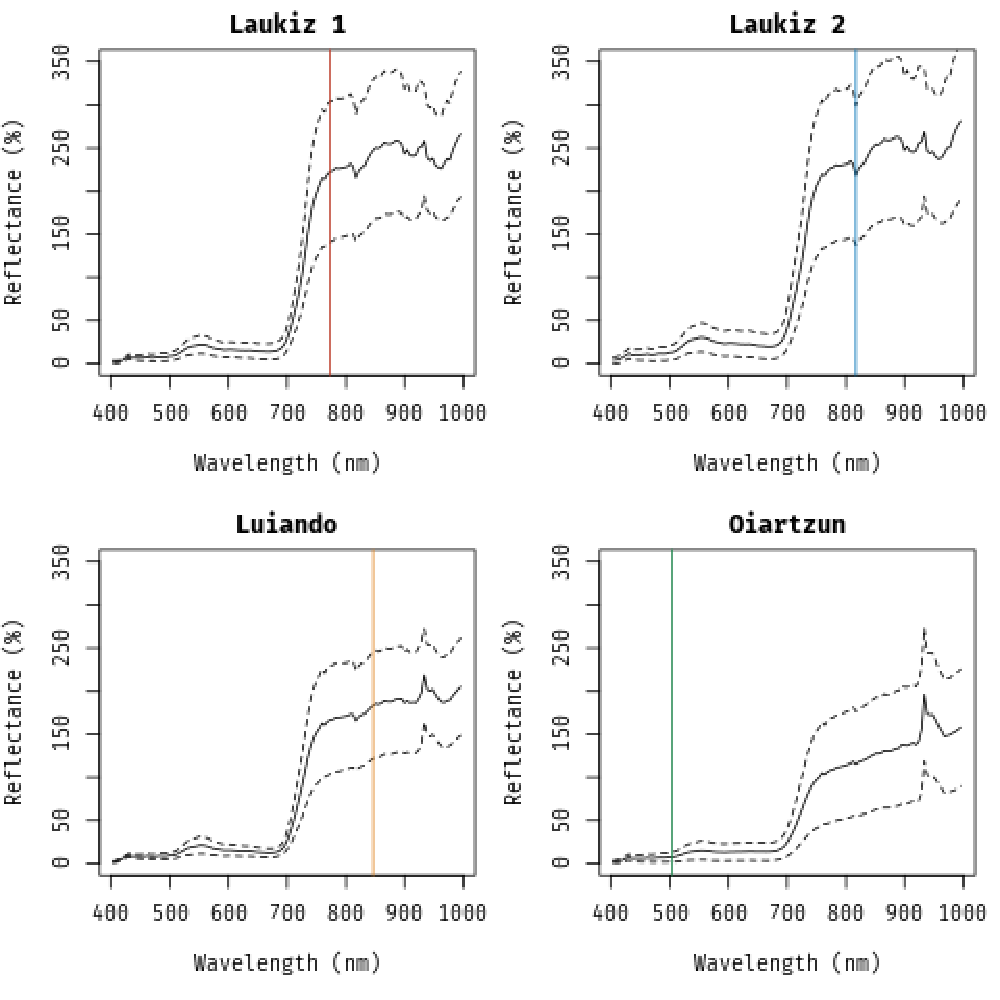
\includegraphics[width=\textwidth] {../03_figures/results/spectral_signatures.pdf}}
		\caption{Spectral signatures (mean and standard deviation) of each plot.
			The colored lines show the most important band for each plot, respectively: Band 80 (773nm, red), band 89 (817nm, blue), band 95 (846nm, orange), band 23 (503nm, green).}
		\label{fig:spectral_signatures}
	\end{center}
\end{figure}

Luiando shows the highest defoliation ($\bar{x} = 68.36 \%$) among the plots while Laukiz 2 is the healthiest ($\bar{x} = 17.73 \%$) (\autoref{fig:defol_boxplots}).
Laukiz 1 and Oiartzun both show a medium defoliation level around 50 \%.
Oiartzun consists mainly of trees that show either a very high level of defoliation ($70 \% <=$) or none at all.
Laukiz 1 shows an evenly distributed level of defoliation across the entire plot.

The high defoliation level of Luiando and Oiartzun is also visible in the spectral signatures of the plots (\autoref{fig:spectral_signatures}).
Both plots show lower mean reflectance values around the wavelength range 800 nm - 1000 nm compared to Laukiz 1 and Laukiz 2.
Oiartzun is almost completely missing the reflectance drop at around 815 nm that is visible for all other plots but instead shows a higher magnitude for the reflectance increase at around 920 nm.
Laukiz 2 shows a mean tree density of 62.51 m \autoref{fig:rmse_defol_dens}) while all other plots are more dense (34.35 (Laukiz 1), 33.77 (Luiando), 35.02 (Oiartzun)) (\autoref{fig:rmse_defol_dens}).

\subsection{Predictive performance}

\begin{table}[t!]
\centering
\caption[t]{Predictive performance of \ac{RR} using the merged dataset (supermodel) and observations on a plot level only (single plot) with \ac{RMSE} as the error measure. The values for "merged dataset" correspond to the fold for which the respective plot was serving as the test set. For "single plot", the values correspond to the mean value of the SpCV at the repetition level (10 folds, 20 repetitions).}
\begingroup\footnotesize
\begin{tabular}{lll}
	\\
	Plot/Data & Merged dataset (Block CV) & Single plot (SpCV) \\
	\hline
	Laukiz 1  & 58.95                     & 89.89              \\
	Laukiz 2  & 27.94                     & 30.37              \\
	Luiando   & 69.72                     & 76.02              \\
	Oiartzun  & 58.09                     & 106.65             \\
	\bottomrule
\end{tabular}
\endgroup
\label{tab:supermodel_performance}
\end{table}

\ac{RR} shows the lowest error for three out of four plots (for Luiando \textit{elasticnet} shows a slightly better performance) (\autoref{tab:penalty_comparison}).
The magnitude of difference for \ac{RR} compared to the other penalties for the plots in which \ac{RR} showed the best performance ranges between XX and XX percent.
For the merged dataset, all penalties show a similar mean predictive performance that outperform all single plot models besides the Laukiz 2 model.

% single models vs supermodel
When comparing the mean predictive performance of the plot level model against the performance of the super model at the plot level (when the respective plot served as the test set), the supermodel also outperforms the Laukiz 2 model (27.94 vs 30.37 RMSE) (\autoref{tab:supermodel_performance}).

The worst performance of the supermodel on the fold level is reported for Luiando (69.72 RMSE) while for the single plot models Oiartzun shows the highest error (106.65 RMSE).

% RMSE vs CV and point dens
Laukiz 2 showed contrary results compared to all other plots when linking \ac{RMSE} against coefficient of variation and mean point density (\autoref{fig:rmse_defol_dens}).
Comparing RMSE against $CV/skewness$ shows a $log_{2}(-x)$ relationship.

% rmse vs defol and point dens
\begin{figure} [b!]
	\begin{center}
		\makebox[\textwidth]{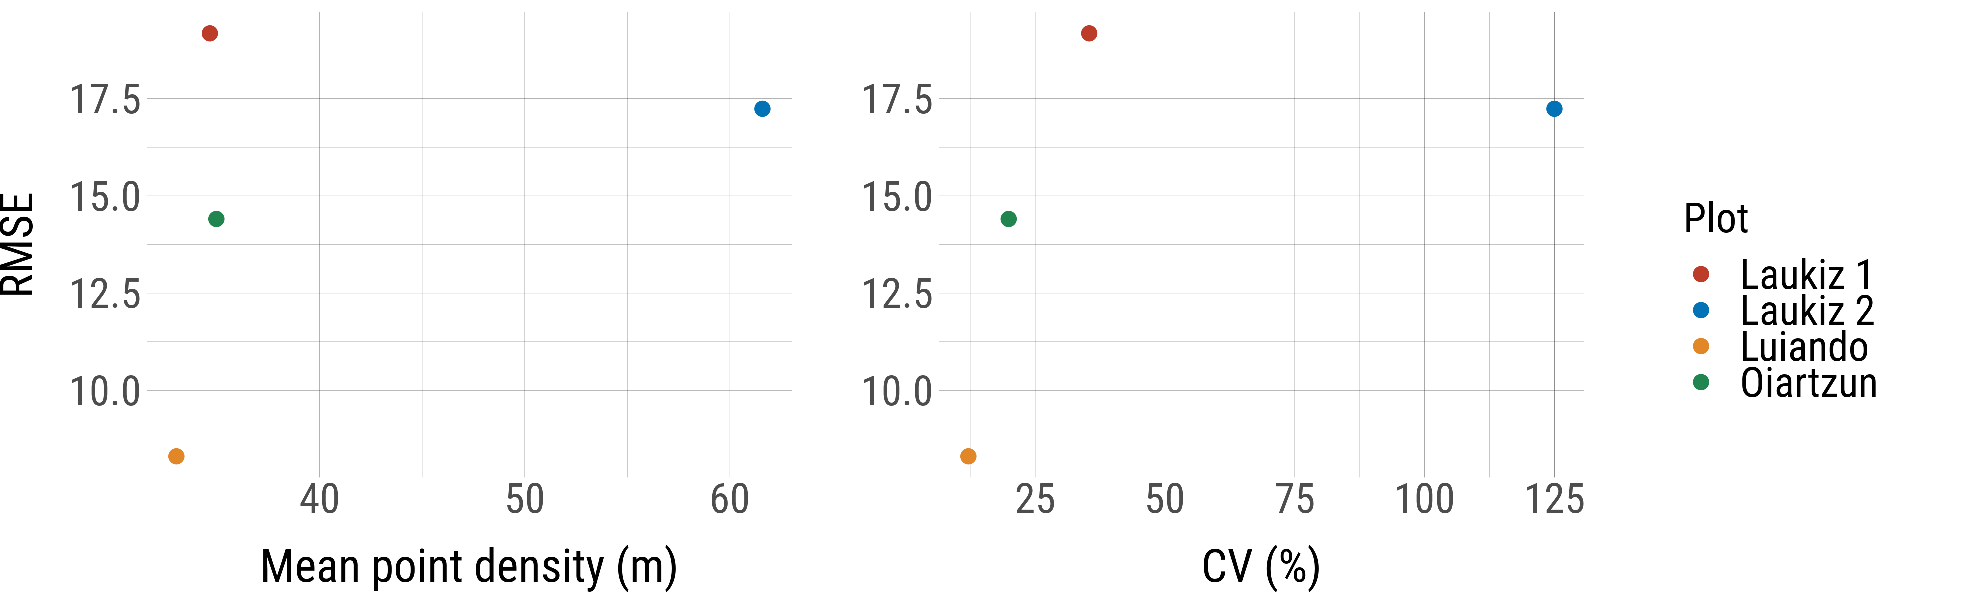
\includegraphics[width=\textwidth] {../03_figures/results/plot-characteristics.pdf}}
		\caption{RMSE vs. mean point density, coefficient of variation and coefficient of variation / skewness.}
		\label{fig:plot-characteristics}
	\end{center}
\end{figure}

\subsubsection{Variable importance}

\ac{NRI}s using bands in the wavelength range of 770 nm - 820 nm (band 80 - band 89), which belongs to the infrared region, appear most often among the ten highest coefficient estimates across all plots (\autoref{tab:variable-importance}).
Only one vegeation index (Datt3) showed up among the most important predictors (Laukiz 1).
Luiando and Oiartzun also prefered bands with longer (938.39 nm (band 114) - 996.31 nm (band 126)) and shorter wavelengths (480.30 nm (band 18) - 503.26 (band 23)).
The first range again belongs to the infrared region while the second is within the region of the visible light, transitioning from blue to green.

% variable importance
\begin{table}[b!]
\centering
\caption[t]{The ten highest coefficient estimates for every plot and the merged dataset.}
\begingroup\footnotesize
\begin{tabular}{lllll}
	\\
	Laukiz 1           & Laukiz 2           & Luiando             & Oiartzun            & All Plots          \\
	\hline
	b80-b77 (0.0089)   & b89-b84 (0.0093)   & b95-b93 (1.5e-36)   & b23-b18 (-0.0090)   & b78-b77 (0.058)    \\
	b81-b77 (0.0079)   & b89-b87 (0.0086)   & b109-b106 (1.4e-36) & b23-b19 (-0.0074)   & b115-b113 (0.054)  \\
	b78-b77 (0.0079)   & b89-b88 (0.0086)   & b92-b95 (1.4e-36)   & b99-b98 (0.0073)    & b82-b77 (0.052)    \\
	b77-b76 (-0.0078)  & b108-b104 (0.0084) & b114-b6 (-1.2e-36)  & b23-b20 (-0.0070)   & b79-b77 (0.049)    \\
	b79-b77 (0.0077)   & b89-b85 (0.0083)   & b96-b93 (1.2e-36)   & b10-b8 (-0.0063)    & b80-b77 (0.049)    \\
	Datt3 (-0.71)      & b92-b84 (0.0083)   & b116-b6 (-1.2e-36)  & b102-b98 (0.0062)   & b81-b77 (0.049)    \\
	b41-b25 (0.0070)   & b89-b83 (0.0081)   & b114-b5 (-1.2e-36)  & b124-b115 (0.0062)  & b81-b78 (-0.048)   \\
	b116-b113 (0.0068) & b89-b86 (0.0080)   & b115-b114 (1.2e-36) & b23-b15 (-0.0060)   & b124-b115 (-0.047) \\
	b82-b77 (0.0068)   & b92-b88 (0.0080)   & b95-b91 (1.1e-36)   & b126-b115 (-0.0060) & b23-b20 (-0.047)   \\
	b77-b75 (-0.0068)  & b108-b96 (0.0079)  & b114-b8 (-1.1e-36)  & b118-b115 (-0.0059) & b80-b78 (-0.046)   \\
	\bottomrule
\end{tabular}
\endgroup
\label{tab:variable-importance}
\end{table}

% band importance
\begin{figure} [b!]
	\begin{center}
		\makebox[\textwidth]{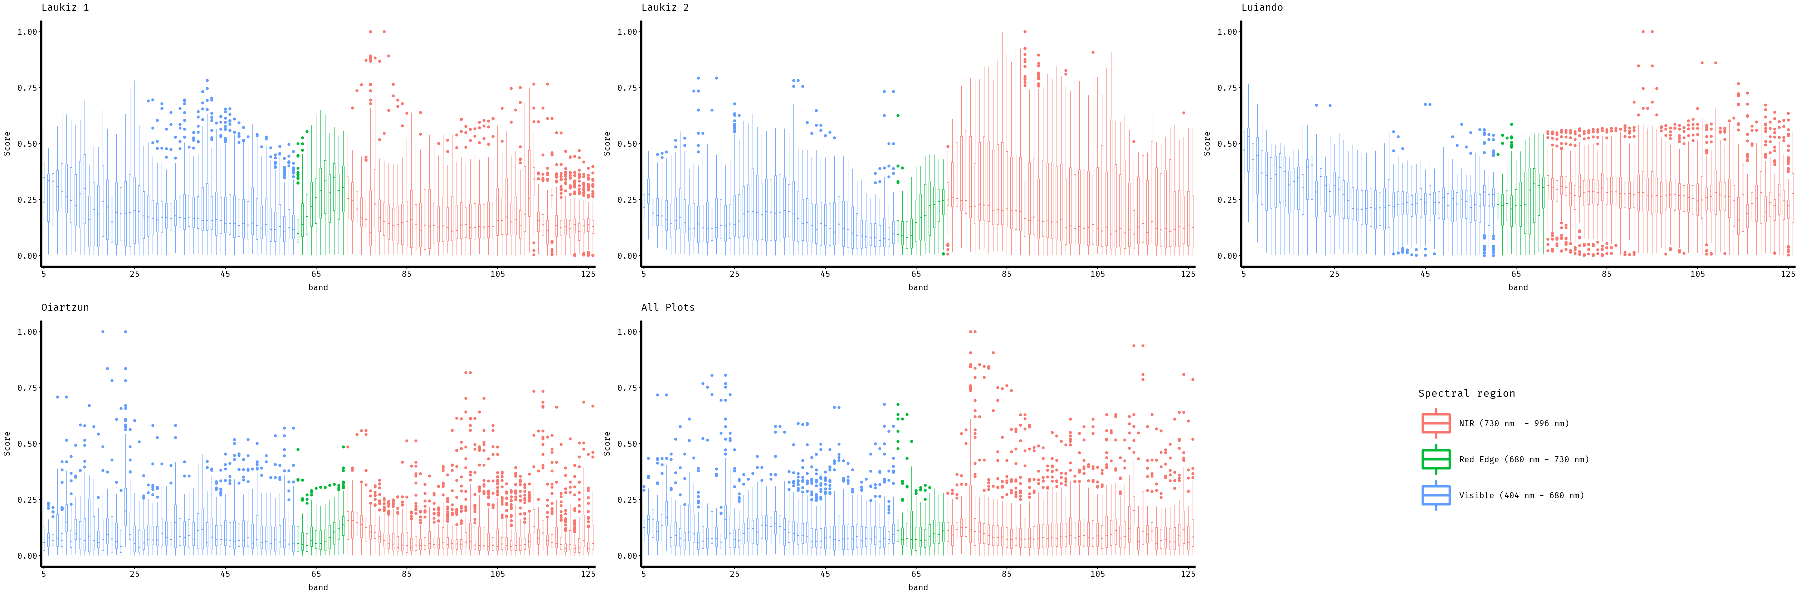
\includegraphics[angle=90, height = 0.95\textheight] {../03_figures/results/important-bands_boxplot.pdf}}
		\caption{test}
		\label{fig:important-bands}
	\end{center}
\end{figure}

\section{Discussion}

\subsection{Index derivation}

The exact number of contributing pixels to the final index value of an observations cannot be determined as it depends on the location of the tree within the pixel grid.
If a tree is located at the border of a pixel, a buffer of e.g. three meters will include more pixels than if the point is located at the center of a pixel.
Also, if a tree is located at the border of the plot, some directions of the buffer will not contain image values.

\subsection{Plot characteristics}

For Laukiz1, Luiando and Oiartzun \ac{RMSE} seems to increase with a higher point density at a first glance.
However, the point densities of these plots are very similar (33.7 m - 35.01 m) and should be interpreted as a group instead of single values.
With Laukiz2 being completely off from the other plots in terms of mean point density, no pattern can be extracted from this result.
Linking RMSE vs coefficient of variation shows the same relationship as linking against mean point density.
The interesting $log_{2}(-x)$ relationship for RMSE vs. coefficient of variation / skewness should be interpreted with caution: The sample size of four plots is not representative to make general statements here.
This finding should be verified with more observations in future studies.

\subsection{Variable importance}


\section*{References}

\bibliography{Biblio_hyperspectral}

\end{document}
